% TEMPLATE for Usenix papers, specifically to meet requirements of
%  USENIX '05
% originally a template for producing IEEE-format articles using LaTeX.
%   written by Matthew Ward, CS Department, Worcester Polytechnic Institute.
% adapted by David Beazley for his excellent SWIG paper in Proceedings,
%   Tcl 96
% turned into a smartass generic template by De Clarke, with thanks to
%   both the above pioneers
% use at your own risk.  Complaints to /dev/null.
% make it two column with no page numbering, default is 10 point

% Munged by Fred Douglis <douglis@research.att.com> 10/97 to separate
% the .sty file from the LaTeX source template, so that people can
% more easily include the .sty file into an existing document.  Also
% changed to more closely follow the style guidelines as represented
% by the Word sample file. 

% Note that since 2010, USENIX does not require endnotes. If you want
% foot of page notes, don't include the endnotes package in the 
% usepackage command, below.

% This version uses the latex2e styles, not the very ancient 2.09 stuff.
\documentclass[letterpaper,twocolumn,10pt]{article}

\usepackage{usenix}
\usepackage{epsfig}
\usepackage{url}
\usepackage{float}
\usepackage{caption}
\usepackage{subcaption}
\usepackage{hyperref}

\hypersetup{
    colorlinks,
    citecolor=black,
    filecolor=black,
    linkcolor=black,
    urlcolor=black
}

\newenvironment{packed_enum}{
\begin{enumerate}
  \setlength{\itemsep}{1pt}
  \setlength{\parskip}{0pt}
  \setlength{\parsep}{0pt}
}{\end{enumerate}}

\newenvironment{packed_item}{
\begin{itemize}
  \setlength{\itemsep}{1pt}
  \setlength{\parskip}{0pt}
  \setlength{\parsep}{0pt}
}{\end{itemize}}

\newenvironment{packed_desc}{
\begin{description}
  \setlength{\itemsep}{1pt}
  \setlength{\parskip}{0pt}
  \setlength{\parsep}{0pt}
}{\end{description}}

\begin{document}

%don't want date printed
\date{}

%make title bold and 14 pt font (Latex default is non-bold, 16 pt)
\title{\Large \bf Custos: A Flexible Cloud ``Key Storage as a Service'' Platform}

%for single author (just remove % characters)
\author{
{\rm Andy Sayler}
\and
{\rm Dirk Grunwald}\\
University of Colorado, Boulder
\and
{\rm Eric Keller}
% copy the following lines to add more authors
% \and
% {\rm Name}\\
%Name Institution
} % end author

\maketitle

% Use the following at camera-ready time to suppress page numbers.
% Comment it out when you first submit the paper for review.
%\thispagestyle{empty}

\subsection*{Abstract}

The magnitude of the digital data we create, store, and interact with
on a daily basis is rapidly increasing. Simultaneously, we are
demanding increasingly diverse use cases for our data: from spreading
it across a variety of services and devices to sharing it with a
number of organizations and friends. Securing our data and controlling
who can access it is thus increasingly important, but also
increasingly difficult. The existing tools we have for protecting our
data, file encryption systems, are extremely inflexible. This
inflexibility is due to encryption key storage being too tightly
coupled with existing data encryption solutions. This tight coupling
makes these systems unusable for many of our desired use cases,
leading to the underutilization of strong encryption and the
associated lack of protection and control of our data. We believe that
this issue can be solved by providing a ``Key Storage as a Service''
system that separates secure key storage and access control from the
underling encryption mechanisms. Toward this end, we present Custos: a
flexible Cloud-based key storage and access control service.

\section{Introduction}
\label{sec:intro}

Today, we use systems like Dropbox~\cite{dropbox} or Amazon
S3~\cite{amazon-s3} to store and sync our files while allowing access
from a variety of end points, but few existing encryption schemes
support this usage. When we wish to transfer and share files, we often
do it via e-mail attachments, removable media, or cloud ``locker''
services, but these forms of ``out-of-band'' sharing are not supported
by most existing secure storage systems. Many of our modern (and
legacy) computing services are designed to run in the background,
devoid of interactive input, but most existing encryption solutions
require interactive input in order to securely access encrypted
files. The inability of existing encryption systems to accommodate the
diverse range of use cases we require leads to such systems being very
difficult to use. This inflexibility is not due to the underlying
encryption itself, but to the methods by which encryption keys are
managed and stored. Today, most file encryption solutions tightly
couple key storage with the underlying encryption. This is a mistake
that has lead to a growing usability gap, and the corresponding
underutilization, of encryption as a tool for securing and controlling
our data \cite{Whitten1999, Sweikata2009, Kher2005, Geambasu2011}.

We propose separating key storage and access management from the
underlying encryption scheme through a ``Key Storage as a Service''
system. Such a service can make encryption systems far more flexible
and accommodating of the diversity of modern use cases, and by
extension, can make file encryption far easier to use. Strong
encryption is one of the best available tools for securing and
protecting our data. We wish to reclaim it as a viable option for
controlling our data in environments that are increasingly outside of
our control.

\begin{figure}[!tb]
  \centering
  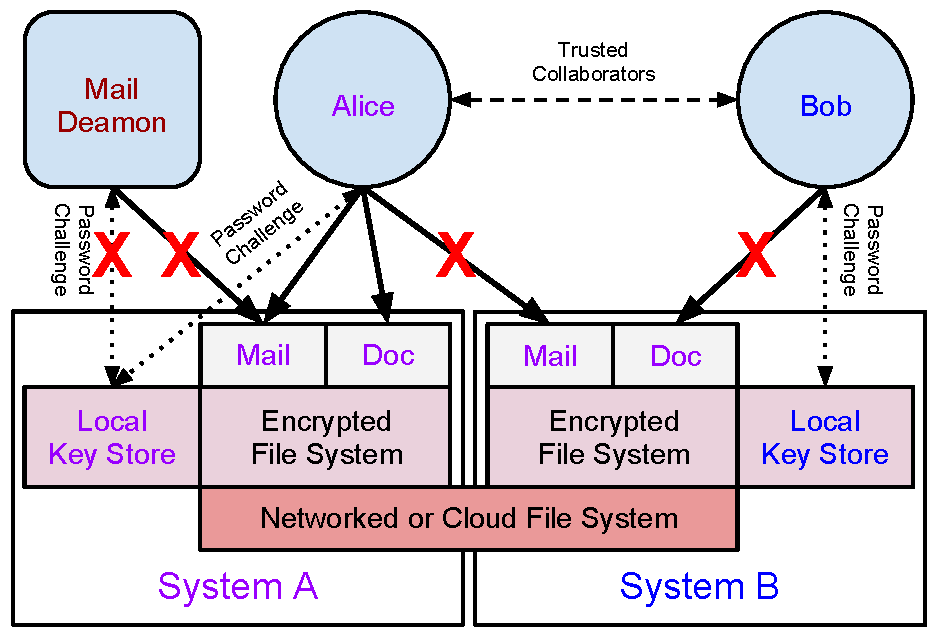
\includegraphics[width=\columnwidth]{./include/Problem-Layered.pdf}
  \caption{Existing Local Encrypted File Systems}
  \label{fig:problem-layered}
\end{figure}

Existing local encrypted file system solutions like
dm-crypt~\cite{dm-crypt} and eCryptfs~\cite{Halcrow} suffer from a
number of limitations related to their tightly-coupled local key
storage and access management components. As Figure
\ref{fig:problem-layered} shows, these systems work fine for an
individual user like Alice wishing to secure items like her mail or
documents and access them from a single machine. But they quickly
break down when trying to move beyond the simple single-user,
single-device use case. Alice can not access her encrypted mail file
across a networked file system from System B since System B has no
access to the encryption keys stored on System A. Furthermore, she can
not share a work document with a trusted collaborator like Bob, since
Bob neither has access to her encryption keys stored on System A nor
the password required to unlock these keys. A non-interactive process
like the Mail Daemon is also unable to leverage these encrypted file
systems due to the inability of such services to securely and
interactively provide a password to unlock the keys needed to decrypt
local files.

\begin{figure}[!tb]
  \centering
  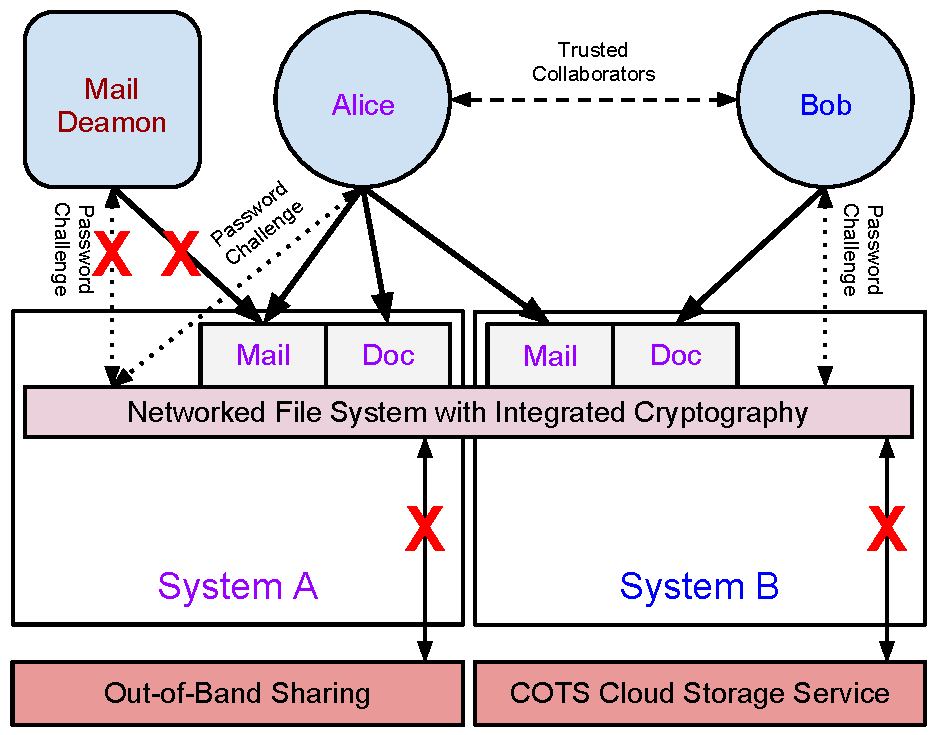
\includegraphics[width=\columnwidth]{./include/Problem-Integrated.pdf}
  \caption{Existing Distributed Encrypted File Systems}
  \label{fig:problem-integrated}
\end{figure}

While distributed encrypted file systems such as
OceanStore~\cite{Kubiatowicz2000}, Plutus~\cite{Kallahalla2003},
Cumulus4j~\cite{cumulus4j}, or Tahoe~\cite{Wilcox-O'Hearn2008} tend to
succeed in solving some of the sharing and distribution problems
inherent in local secure file systems, they still lack the flexibility
required to address the full range of desired use cases. Figure
\ref{fig:problem-integrated} shows some of the remaining issues
inherent in distributed solutions. Notably, while multi-user use cases
are better supported, non-interactive use cases are still a
challenge. Furthermore, full stack distributed file systems tend to be
wedded with specific storage systems and thus lack support for
Cloud-based Storage as a Service offerings or alternate underlying
storage technologies. These systems also lack support for most forms
of ``out-of-band'' file sharing (via e-mail, USB flash drives, etc)
due to the inability of actors outside of the integrated stack to
access the necessary encryption keys.

Existing systems force the user into a very specific security model,
appropriate for certain use cases, but useless for many others. These
systems also only support to a handful of technologies often excluding
alternate, new, or unforeseen options. They fail to accommodate our
natural usage patterns, and thus often go unused. The solution is to
acknowledge the fact that one-size-does-not-fit-all when it comes to
securing our data. And then to build a system around this principle,
capable of supporting an extensible range of use cases. Toward this
end we present Custos: a flexible ``Key Storage as a Service'' system
designed to support a variety of data security requirements across a
wide range of use cases. Custos is based on three core principles:

\begin{packed_item}
\item Decoupled Key Storage
\item Flexible Security Models
\item Global Access and Centralization
\end{packed_item}

We propose the following common use-case examples, none of which are
well supported by existing encryption systems, that we believe can be
better supported by using Custos-integrated encryption systems:

\begin{packed_desc}
\item[Secure Multi-Devices Access:] Alice uses Dropbox~\cite{dropbox} to
  synchronize her files between her work computer, her home computer,
  and her tablet. She wishes to encrypt her Dropbox-synced files
  while maintaining the ability to access and modify files across all
  of her devices regardless of the device on which they were created
  or originally encrypted.
\item[Secure Out-of-Band Sharing:] Alice wants to send Bob an
  encrypted file via e-mail attachment or USB flash drive. She wishes
  to grant Bob secure access to the file so that Bob and decrypt and
  read the file easily without requiring a cumbersome manual exchange
  of encryption keys via a phone call or in-person meeting.
\item[Secure Autonomous Access:] Alice has an account on a server
  where she uses a file-level encryption system like
  eCryptfs~\cite{eCryptfs} to encrypt her home directory,
  automatically decrypting her files when she is logged in. Alice has
  a mail forwarding configuration file in her home directory that
  directs the local mail server to forward e-mail sent to this server
  to her primary e-mail account. Thus, she must grant the local mail
  daemon autonomous access to that single encrypted configuration file
  while retaining the interactive log in requirement for access to all
  her other home directory files.
\end{packed_desc}

Through the remainder of the paper we will discuss Custos and how it's
flexibility can accommodate these, and many other, use-case
examples. In \S \ref{sec:principles} we discuss the core Custos
concepts in more depth. We go on to present the architectures of
Custos in \S \ref{sec:arch} as well as our prototype implementation in
\S \ref{sec:implementation}. Finally, we close by discussing the assumed thread
model and limitations of Custos in \S \ref{sec:model} as well as our
conclusions and visions for the future in \S \ref{sec:conclusion}.

\section{Principles of Custos}
\label{sec:principles}

We feel that there are three core principles necessary for
successfully building a usable encryption key storage and access
control system. The absence of these principles in existing data
encryption systems has lead to the usability issues discussed in \S
\ref{sec:intro}. In an effort to address these deficiencies and
provide an alternative, we have designed Custos based around these
core principles.

\subsection{Decoupled Key Storage}

Existing encryption systems almost always bundle their own key storage
and access control components. This practice unnecessarily couples the
authentication and authorization models used to protect encrypted
files with the actual encryption itself. Such a coupling not only
duplicates efforts across a wide range of encryption systems, but also
reduces the user's flexibility to select encryption requirements
separately from her selection of authentication and authorization
requirements.

Custos breaks this unnecessary coupling by providing ``Key Storage as
a Service''. Custos's sole responsibility is to store the keys
required to encrypt or decrypt specific files, and to control who may
access each key. Custos exposes a key access API that provides a
standardized interface through which a variety of file encryption
systems may read, write, add, or delete keys. This allows Custos to
focus on key storage and access management, while individual
encryption systems focus on the actual file encryption. Key storage
and access control is a fundamentally different problem than file
encryption, and it requires a fundamentally separate service-oriented
solution.

\subsection{Flexible Security Models}

Not all data is equal, and neither is the means with which we must
protect it. A highly sensitive personal file has very different
authentication requirements and threat models than a document that is
being composed by a team of trusted collaborating
individuals. Likewise, different systems have different authentication
capabilities. An interactive desktop application can partake in a
separate set of authentication techniques than a non-interactive
autonomous server is capable of using. The methods by which we
authenticate actors wishing to access our data and the authorizations
granted to each actor vary for each file we wish to protect. Any data
encryption system that forces a single authentication model on all
data it is designed to protect is inherently limiting.

Custos strives to overcome this issue by providing a flexible and
extensible authentication and requirements framework capable of
supporting separate access and threat models for each individual
file. Not unlike the Pluggable Authentication Module
(PAM)~\cite{linux-pam} system used in many POSIX operating systems,
Custos supports an extensible authentication and requirements module
framework. Each module requires an actor wishing to access a key in
the Custos system to satisfy a particular set of requirements before
being allowed to proceed with its access request. Modules can be used
to impose both authentication requirements on requesting actors as
well as ``process'' requirements on client file systems. An example of
the later would be requiring a new key to be provided with each file
access in situations where forced re-keying of encrypted data is
desirable. Each key in the Custos system has an associated module or
list of modules that must be satisfied by the actor prior to being
granted access to the key. Modules may be enabled, disabled, or
chained together on a per-key basis. This system provides the user
with a wide range of flexibility in selecting which access and threat
models are appropriate for a particular file: allowing Custos to
support a variety of use cases on the security vs accessibility
spectrum.

\subsection{Global Access and Centralization}

The modern Internet not only allows us to move and share data at
levels never before possible, in many instances it requires it. Our
data is no longer limited to a single machine, or even a single
user. It is highly mobile and often shared. We are used to storing our
data in globally accessible locations (e.g. the Cloud) or
synchronizing it across machines so that we may access it from a
variety of devices in a variety of situations. Furthermore, sharing
data with other users via a myriad of means (e-mail, file lockers,
etc) is a natural and everyday occurrence. The key storage and access
control mechanisms built into existing encryption system are not good
at dealing with this lose model of data location or access domain.

Custos addresses these issues via its design as a logically
centralized, globally accessible ``Cloud'' service. Regardless of
where an encrypted file system happens to be running, such systems can
always access Custos via the Internet and attempt to obtain the
encryption keys they require\footnote{This is not to imply that there
  can only ever be a single instance of ``Custos'' available on the
  public Internet. We envision many individuals operating their own
  ``Custos'' servers for practical or compliance related reasons. But
  all of these instance should be accessible from the public Internet,
  facilitating Custos use regardless of location.}. This also extends
to shared data available to multiple users. It does not matter if all
users are located in a single domain or whether or not they can all
make connections to a local trusted server. Any user with access to
the Internet can request access to a key via Custos\footnote{The
  principle that any user on the Internet should be able to request
  access to any Custos-held key by no means implies that this request
  should always be granted. The authentication and requirements
  modules associated with each key will dictate the response to such a
  request. But global accessibility ensures that access control
  limitation are imposed by intentionally crafted policies and not by
  limitations in the key storage system.}.

In addition to global accessibility, the logically centralized nature
of Custos provides it with audit, logging, and centralized management
capabilities. Since access to an encrypted file must by nature begin
with a Custos request for the associated key, Custos can be configured
to log these requests. These logs may then be used to audit file
access, revealing when and by which authentication means actors are
accessing Custos-protected files. In addition to logging, Custos's
centralized nature also makes it a simple choke point at which access
to encrypted files distributed across a multitude of devices can by
revoked or modified without needing to modify the files at each
location directly. As suggested in \cite{Geambasu2011}, this
capability can prove very useful in cases where devices storing data
are lost or stolen, allowing the data to be effectively ``deleted''
(or at least rendered unreadable) via the deletion of the associated
centrally-managed encryption key.

% Andy's Note: IS it worth addressing the somewhat in-depth point that
% this form of key-based access logging and ``deletion'' only applies
% to the access of a file on a securely implement client-system
% (i.e. non key caching, etc)? Yes, an adversely-designed Custos
% client only needs to hit Custos once per file, after which it can
% either store a decrypted copy of the file or a local copy of the
% key. But for the user wishing to secure their own data, a client
% that avoids these behaviors would still allow key-based file access
% revocation and logging in the event that the legitimate user losses
% control of the device. Since we assume users wishing to use
% encryption in the first case are also committed to the security of
% their own data, I don't know that the adversarial-client'' threat
% vector necessarily needs to be addressed at this time. Any user
% wishing to employ an adversarial client might as well just forgo
% using encryption in the first place...

\section{Custos Architecture}
\label{sec:arch}

As discussed in \S \ref{sec:principles}, Custos is built around three
core principles. In this section, we look at the architecture we've
designed to realize these principles. Figure \ref{fig:custosoverview}
shows the basic block diagram for Custos and how it might integrate
with existing encrypted file systems. We discuss these components in
detail in this section.

\begin{figure}[!tb]
  \centering
  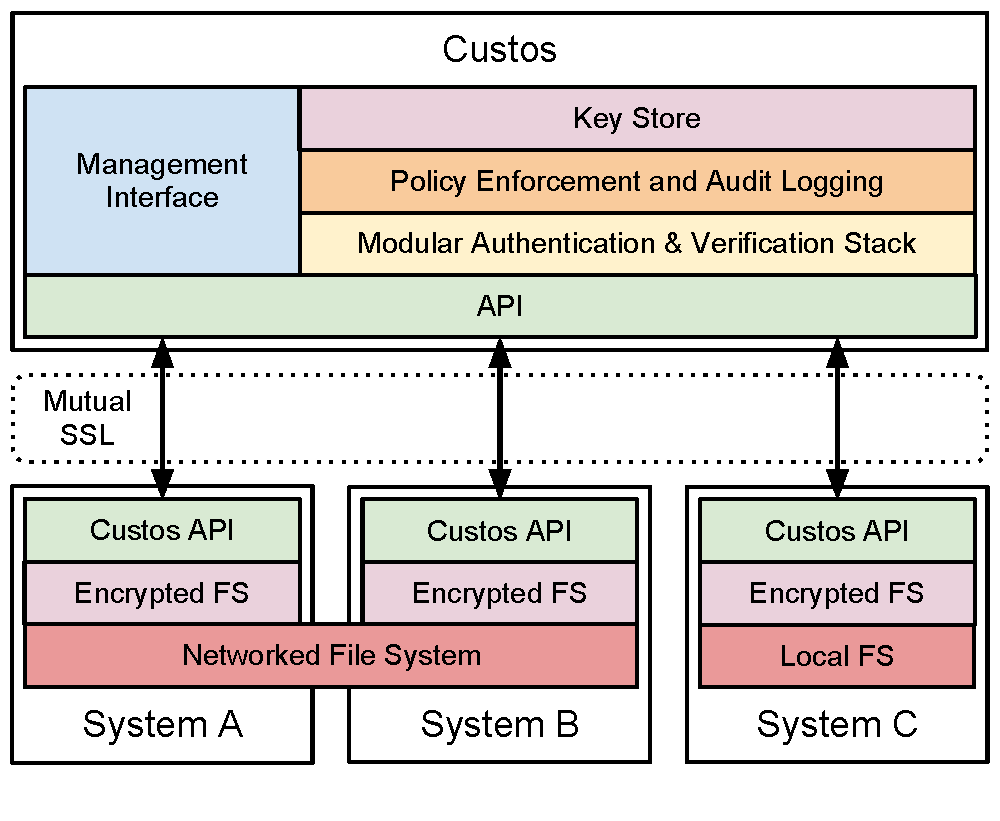
\includegraphics[width=\columnwidth]{./include/CustosOverview.pdf}
  \caption{Custos Architecture Overview}
  \label{fig:custosoverview}
\end{figure}

\subsection{Custos Key Request API}

The Custos Key Request API is the means by which encryption systems
access Custos. Through this API, Custos-integrated encryption systems
may perform operations like adding, deleting, accessing, or modifying
keys. We assume that Custos will primarily be used to store per-file
symmetric encryption keys, as symmetric keys and the encryption
methods associated with them provide the greatest degree of
flexibility for controlling file access on a per-file level. As such,
each key in Custos is mapped to the UUID of the file it was used to
encrypt. It is up to each encrypted file system to store the Custos
UUID for each file, but this is easily accomplished through the use of
file system provided extended attributes or separate databases. When a
system wishes to access or modify the key for a particular file in
Custos, it makes a call to the Custos API, providing the UUID for the
file in question as part of the request. In response, Custos will
establish a connection with the requesting system and request any
additional information required to authenticate the associated
actor. If the actor can be properly authenticated, and if Custos
determines that they are authorized to access the file, then Custos
will provide the key in question. Because the key exchange process
must be secure, we envision all Custos API interaction occurring over
a mutually-authenticated SSL connection or similar
bidirectionally-secured communication channel.

\subsection{Custos Authentication Modules}

\begin{figure}[!tb]
  \centering
  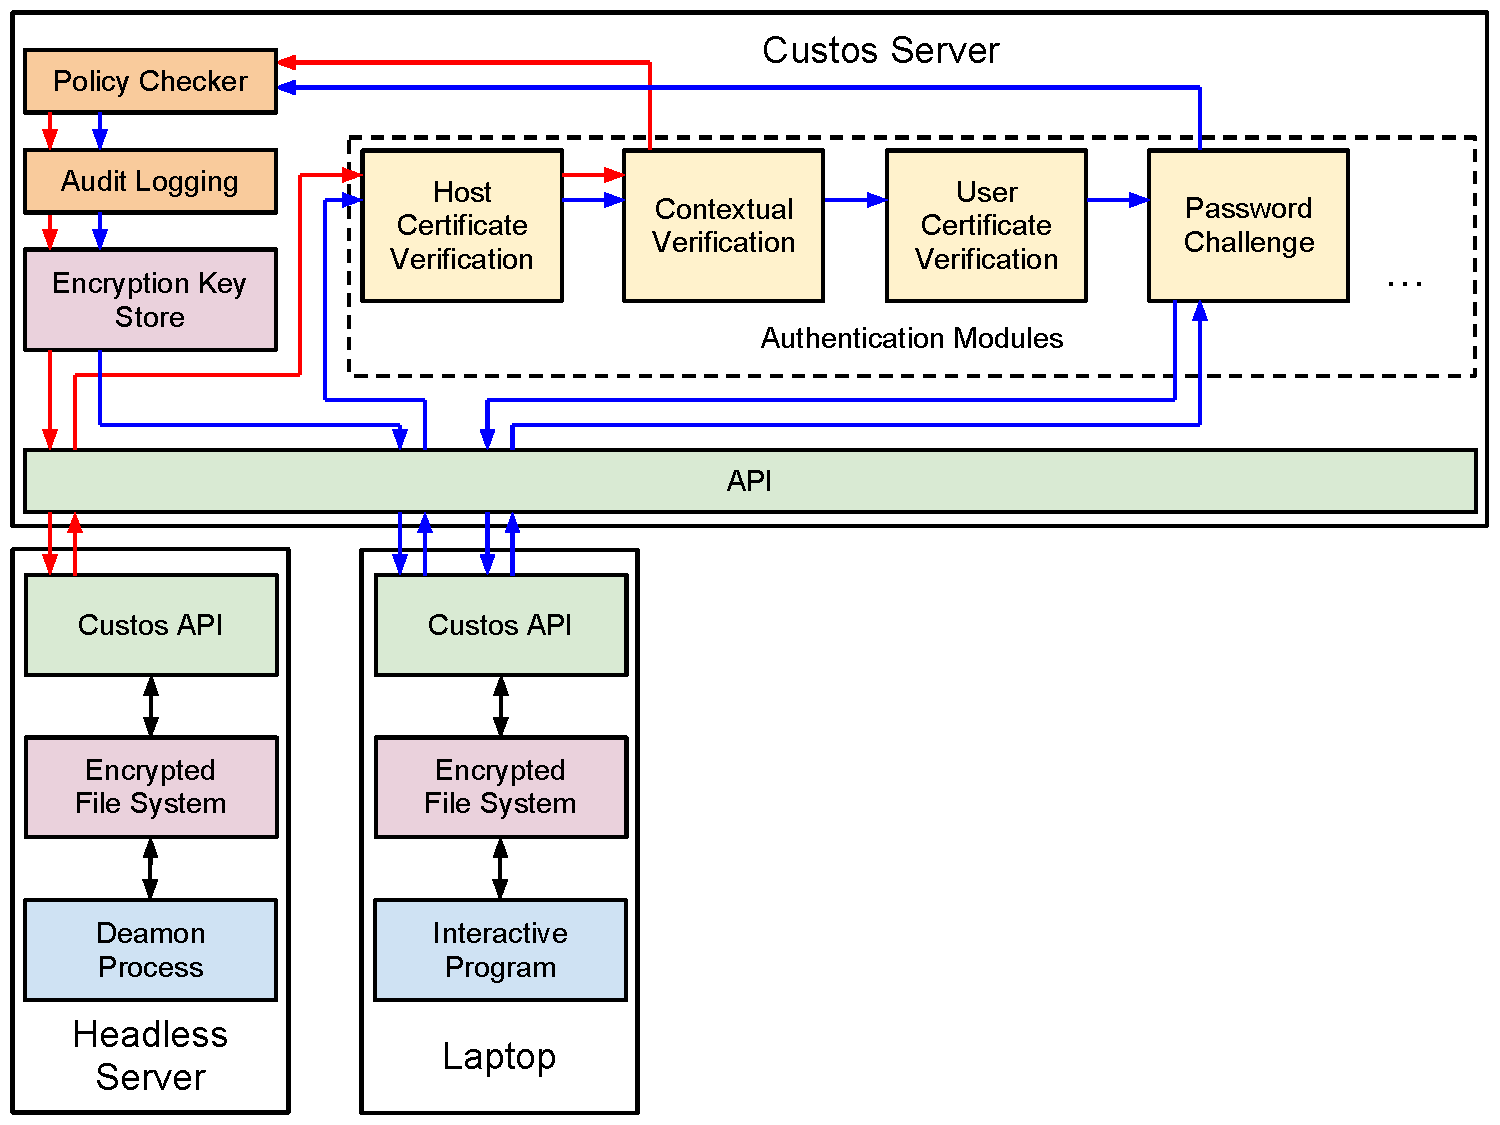
\includegraphics[width=\columnwidth]{./include/KeyRequest.pdf}
  \caption{Custos Key Request Examples}
  \label{fig:keyrequest}
\end{figure}

At Custos's core is its flexible support for a variety of
authentication and requirement modules. Custos provides a standardized
framework for adding modules. Each module verifies a specific
authentication or related requirement. Multiple modules can be chained
together in order to force Custos clients to meet multiple
requirements. Each key in Custos is associated with one or more module
chains, and access to that key will only be provided to clients that
can properly satisfy all modules in at least one valid chain. By
allowing multiple chains to be defined for each key, Custos enables
easy key sharing where different users can be required to supply
separate passwords, certificates, etc to access the same key. Custos
provides a handful of common modules by default, but also makes it
easy for users to add modules as needed via the extensible module
interface.

Since the Custos module system is at the heart of Custos's
flexibility, we envision using modules for a variety of authentication
methods. These include interactive authentication modules like simple
password-challenge modules that require the requesting actor to
provide a valid password or multi-factor-challenge modules that
require the user to posses a separate security device. They also
include non-interactive modules like public-private key modules to
authenticate specific actors or contextual security modules that place
limits on which network locations actors may access keys from, what
times of day keys can be accesses, or other environmental context
restraints \cite{Hulsebosch2005}. This range of modules, and the
ability to mix-and-match them to form separate authentication
requirements for each Custos key allows Custos to provide secure key
access in the widest possible variety of situations. For example,
Figure \ref{fig:keyrequest} shows two separate systems utilizing
Custos to access the required encryption keys to decrypt files on each
system. In the case of the Headless Server, only non-interactive
security modules are required for authentication, allowing a daemon
background process on the server to securely access an encrypted file
autonomously without requiring interactive human intervention. The
laptop, on the other hand, provides additional security by requiring
both interactive and non-interactive authentication methods,
appropriate for the protection of personal data that is only ever
accessed by a live user.

\subsection{Custos Management Interface}

Custos also provides a management interface via an additional API. We
envision such an API allowing for the easy construction of both web,
desktop, and command line based interfaces for managing Custos. The
management interface allows the Custos administrator to specify
authentication module chains for each key, to manually add, remove, or
modify keys, to revoke key access (as in the case of a stolen laptop,
etc), and to access the audit logs for a given key. This interface is
also where the settings for each module instance (shared secrets,
public keys, etc) are configured. Custos allows the user to define a
default authentication module chain that is automatically attached to
new keys as they are created. Per-file requirements that differ from
the default are then configured via the management interface. It is
important to note that this management interface is separate from the
Custos key access interface. We wish to encourage the separation of
authentication and access policy (controlled via the management
interface) from the underlying use of each key (via the key access
interface). This separation of policy and mechanism has proven
valuable in a variety of other systems, and we feel it serves Custos
well.

\section{Conclusions and Future Work}
\label{sec:conclusion}

Encryption key storage is too tightly coupled with existing encrypted
file system solutions. This tight coupling makes these systems
inflexible and thus unsuitable for many of our required use cases.
Such inflexibility leads to the underutilization of data encryption by
vast portions of the user base at a time when encryption is becoming a
more and more important tool for retaining control of our data. We
believe that this issue can be solved by providing a ``Key Storage as
a Service'' system that separates encryption key storage and access
control from the underlying encryption mechanisms that use these
keys. Custos provides this flexible Cloud-based key storage service.

We are currently working on building a full Custos prototype that
integrates with a basic encrypted file system~\cite{sayler-os-encfs}
built atop the Linux FUSE API. We hope to use this prototype to refine
the structure of both the management and key access APIs and to prove
out our modular authentication and requirements framework. Going
forward, we hope to provide example Custos integrations with a variety
of existing secure file systems, from systems like eCryptfs to systems
like OceanStore. We plan to use these implementations to demonstrate
how Custos can extend the flexibility and usability of a variety of
encryption solutions across a variety of use cases. We also plan to
further analyze the threat vectors inherent to a ``Key Storage as a
Service'' system and provide suggestions for practically mitigating
these threats in Custos deployments. We have plans to explore a
multi-provider Custos system that reduces the trust required for each
Custos server in favor of distributing portions of each key across
multiple servers. We hope to investigate the usability of Custos in a
variety of real-world use cases.


{
\footnotesize
\bibliographystyle{acm}
\bibliography{refs.bib}
}

\end{document}
